% Provenance (never printed): old terminale S material on mountain ranges and
% continental collision (folds, reverse faults and nappes as signs of
% shortening and thickening; ophiolites and sutures as the trace of a closed
% ocean; the Himalaya and the Alps as examples). Owner (Sync 0): collision,
% fold/anticline/syncline/fold axis, reverse fault/thrust, nappe, ophiolite,
% suture, shortening. Fault is Book 1's (g7), normal fault g11.05's, the root
% and Airy isostasy g11.03's and g12.01's: recalled, never redefined. India's
% past latitudes: figdata/grade-12/india_drift.py (GPlates Web Service, two
% published plate models); shortening: figdata/grade-12/fold_shortening.py;
% the belt map: figdata/grade-12/alpine_belt.py.
\chapter{La formation des montagnes}\label{ch:g12:mountain-building}

Les alpinistes qui atteignent le sommet de l'Everest, à \qty{8848.86}{m}
au-dessus du niveau de la mer, se tiennent sur du calcaire. Les géologues
qui ont redescendu des échantillons du sommet y ont trouvé des fragments de
trilobites, d'ostracodes et de crinoïdes~: des animaux marins qui vivaient
il y a plus de 440 millions d'années, à l'Ordovicien. La plus haute roche
du monde s'est déposée au fond d'une mer. Ce chapitre explique comment un
fond marin finit sur le toit du monde~: deux continents entrent en
collision, et la croûte prise entre eux est comprimée, plissée, empilée et
épaissie jusqu'à former une chaîne de montagnes.
% ledger: sakai05:summit, tulane:roots (marine limestones at the top of Mt. Everest), ics:base.Ordovician, ics:base.Silurian (486.85-443.1 Ma); Book 1: tht:everest (8848.86 m)

\begin{omfigure}
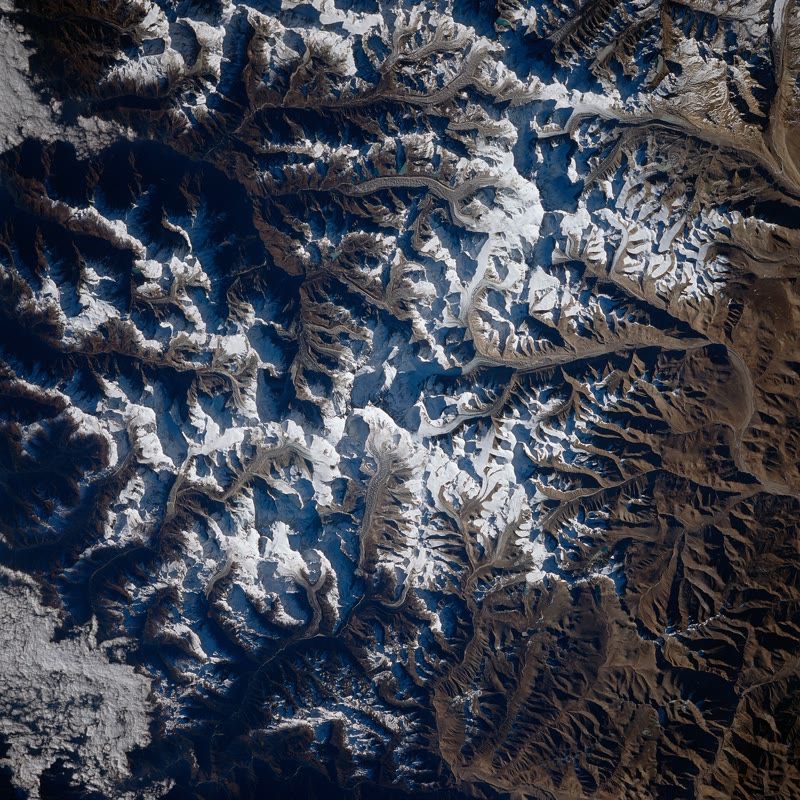
\includegraphics[width=0.5\linewidth]{images/book2/g12-nasa-everest-columbia.jpg}

{\small L'Everest et les nombreux glaciers qui l'entourent, vus depuis la
navette spatiale Columbia le 30 novembre 1996. Photographie NASA (domaine
public).}
\end{omfigure}
% ledger: photo:g12-everest-columbia

\begin{recall}
Une plaque de \omterm{def:g11:ocean-ridges:oceanic-lithosphere}{lithosphère océanique}, fabriquée à une dorsale, replonge dans
le manteau à une fosse~; son \omterm{def:g11:subduction-zones:slab}{panneau plongeant} la tire vers le bas
(\cref{ch:g11:subduction-zones}). La \omterm{def:g12:continental-crust:continental-crust}{croûte continentale} est épaisse et
légère, environ \qty{2830}{kg/m^3} en moyenne contre \qty{3380}{kg/m^3}
pour le manteau situé dessous~: elle flotte donc haut, et une croûte
épaisse se dresse plus haut qu'une croûte mince, au-dessus d'une \omterm{def:g12:continental-crust:root}{racine}
(\cref{ch:g12:continental-crust,ch:g11:lithosphere-asthenosphere}). Une
faille est une cassure le long de laquelle les deux blocs se sont
déplacés~; à une \omterm{def:g11:ocean-ridges:normal-fault}{faille normale}, le bloc situé au-dessus du plan de faille
est descendu, comme là où la croûte est étirée à une dorsale lente
(\cref{ch:g11:ocean-ridges}).
\end{recall}
% ledger: cm95:crust, data:prem, tulane:no-subduct, usgs:normal-fault

\section{De la subduction à la collision}

Un océan consommé à une fosse plus vite qu'il n'est fabriqué à sa dorsale
rétrécit. Un continent porté par la plaque qui plonge se rapproche de la
fosse à la vitesse de la plaque, et finit par y arriver. La \omterm{def:g11:ocean-ridges:oceanic-lithosphere}{lithosphère
océanique} qui le précédait est descendue~; le continent ne peut pas la
suivre, car sa croûte est trop légère pour s'enfoncer dans le manteau, plus
dense. La \omterm{def:g11:subduction-zones:subduction}{subduction} s'arrête. Les deux continents sont pressés l'un contre
l'autre, et le \omterm{def:g11:subduction-zones:slab}{panneau plongeant} qui pendait sous le fond océanique finit
par se détacher et sombrer dans le manteau.
% ledger: earle:collision, tulane:no-subduct

\begin{definition}[Collision continentale]\label{def:g12:mountain-building:collision}
Une \emph{collision continentale}\index{collision continentale} est la
rencontre de deux continents à une limite de plaques convergente, une fois
que la \omterm{def:g11:ocean-ridges:oceanic-lithosphere}{lithosphère océanique} qui les séparait a été subduite. Aucun des
deux continents ne s'enfonce~: la croûte prise entre eux est déformée et
épaissie en une chaîne de montagnes.
\end{definition}
% ledger: earle:collision, tulane:no-subduct, usgs:himalaya-collision

\begin{omfigure}
\begin{tikzpicture}[x=0.95cm, y=0.95cm, font=\scriptsize]
  % ---- stage 1: the ocean closes ----
  \begin{scope}[yshift=0cm]
    \fill[omSea] (3.4,0) -- (8.6,0) -- (8.0,-0.5) -- (4.3,-0.5) -- (3.5,0.0) -- cycle;
    \fill[omLithGranite] (0,0.15) -- (3.5,0.15) -- (4.3,-0.5) -- (4.3,-0.75) -- (3.5,-1.0) -- (0,-1.0) -- cycle;
    \fill[omLithBasalt] (4.3,-0.5) -- (8.0,-0.5) .. controls (9.0,-0.75) and (9.6,-1.2) .. (10.4,-2.0)
      -- (10.15,-2.15) .. controls (9.4,-1.4) and (8.9,-1.0) .. (8.0,-0.75) -- (4.3,-0.75) -- cycle;
    \fill[omLithGranite] (8.0,-0.5) -- (8.6,0.2) -- (12,0.2) -- (12,-1.05) -- (9.5,-1.05)
      .. controls (9.0,-0.75) .. (8.0,-0.5) -- cycle;
    \fill[omThm!70] (10.0,0.2) -- (10.3,0.55) -- (10.6,0.2) -- cycle;
    \draw[black!60, line width=0.3pt] (0,0.15) -- (3.5,0.15) -- (4.3,-0.5) -- (8.0,-0.5) -- (8.6,0.2) -- (12,0.2);
    \draw[-{Stealth[length=2mm]}, line width=0.8pt] (1.2,0.45) -- (2.6,0.45);
    \node[anchor=east] at (0,-0.4) {1};
    \node at (1.8,-0.5) {continent};
    \node at (6.1,-0.25) {océan};
    \node[anchor=north] at (6.1,-0.8) {lithosphère océanique};
    \node[anchor=south] at (8.0,0.0) {fosse};
    \node[anchor=south] at (10.3,0.55) {arc volcanique};
    \node at (11.1,-0.5) {continent};
  \end{scope}
  % ---- stage 2: the continents meet ----
  \begin{scope}[yshift=-3.0cm]
    \fill[omSea] (6.9,0) -- (8.4,0) -- (8.0,-0.4) -- (7.4,-0.35) -- cycle;
    \fill[omLithGranite] (0,0.15) -- (6.8,0.15) -- (7.6,-0.4) -- (8.0,-0.5)
      .. controls (9.0,-0.75) .. (9.5,-1.05) -- (9.2,-1.4) -- (6.5,-1.0) -- (0,-1.0) -- cycle;
    \fill[omLithBasalt] (9.5,-1.05) .. controls (10.0,-1.4) .. (10.6,-2.0) -- (10.35,-2.15)
      .. controls (9.8,-1.6) .. (9.2,-1.4) -- cycle;
    \fill[omLithGranite] (8.0,-0.5) -- (8.6,0.2) -- (12,0.2) -- (12,-1.05) -- (9.5,-1.05)
      .. controls (9.0,-0.75) .. (8.0,-0.5) -- cycle;
    \fill[omLithPeridotite] (7.0,0.15) -- (7.9,0.15) -- (8.3,0.05) -- (7.95,-0.12) -- (7.3,0.0) -- cycle;
    \fill[omThm!70] (10.0,0.2) -- (10.3,0.55) -- (10.6,0.2) -- cycle;
    \draw[-{Stealth[length=2mm]}, line width=0.8pt] (3.2,0.45) -- (4.6,0.45);
    \node[anchor=east] at (0,-0.4) {2};
    \node at (3.4,-0.45) {continent};
    \draw[black!60] (7.6,0.12) -- (7.0,0.75) node[anchor=south east, inner sep=1pt] {écaille de fond océanique};
    \node at (11.1,-0.5) {continent};
    \node[anchor=west] at (10.7,-1.9) {panneau plongeant};
  \end{scope}
  % ---- stage 3: a mountain belt ----
  \begin{scope}[yshift=-6.4cm]
    \fill[omLithGranite] (0,0.15) -- (4.5,0.15) .. controls (6.0,0.4) and (6.6,1.25) .. (7.6,1.3)
      .. controls (8.7,1.3) and (9.6,0.5) .. (10.6,0.2) -- (12,0.2) -- (12,-1.05) -- (10.6,-1.1)
      .. controls (9.5,-2.2) and (8.6,-2.6) .. (7.7,-2.6) .. controls (6.6,-2.6) and (5.6,-1.6) .. (4.5,-1.0)
      -- (0,-1.0) -- cycle;
    \draw[black!60, line width=0.3pt] (0,0.15) -- (4.5,0.15) .. controls (6.0,0.4) and (6.6,1.25) .. (7.6,1.3)
      .. controls (8.7,1.3) and (9.6,0.5) .. (10.6,0.2) -- (12,0.2);
    \draw[black!60, dashed, line width=0.4pt] (0,-1.0) -- (4.5,-1.0) .. controls (5.6,-1.6) and (6.6,-2.6) .. (7.7,-2.6)
      .. controls (8.6,-2.6) and (9.5,-2.2) .. (10.6,-1.1) -- (12,-1.05);
    \draw[omThm, line width=1.0pt] (7.0,1.25) -- (8.3,-2.55);
    \foreach \t in {0.15,0.4,0.65}
      \fill[omLithPeridotite] ($(7.0,1.25)!\t!(8.3,-2.55)$) ++(-0.12,0.05) -- ++(0.3,0) -- ++(-0.05,-0.22) -- ++(-0.3,0) -- cycle;
    \fill[omLithBasalt] (10.9,-1.9) -- (11.5,-2.35) -- (11.35,-2.5) -- (10.75,-2.05) -- cycle;
    \node[anchor=east] at (0,-0.4) {3};
    \node at (2.4,-0.45) {continent};
    \node at (11.3,-0.5) {continent};
    \draw[black!60] (7.2,0.6) -- (5.9,1.5) node[anchor=east, inner sep=1pt] {suture à ophiolites};
    \node at (7.7,-1.9) {racine};
    \node[anchor=north] at (11.2,-2.5) {panneau détaché};
    \node[anchor=south] at (7.6,1.35) {chaîne de montagnes};
  \end{scope}
\end{tikzpicture}

{\small De la \omterm{def:g11:subduction-zones:subduction}{subduction} à la collision (sans échelle). 1~: un océan se
ferme à mesure que son fond plonge à une fosse. 2~: le continent arrive à
la fosse et ne peut pas s'enfoncer~; des écailles de fond océanique sont
poussées sur son bord. 3~: la croûte prise entre les deux continents est
raccourcie et épaissie en une chaîne de montagnes qui repose sur une
\omterm{def:g12:continental-crust:root}{racine}~; la ligne où les deux continents sont soudés, jalonnée d'écailles
de fond océanique, est la \omterm{def:g12:mountain-building:suture}{suture}~; le \omterm{def:g11:subduction-zones:slab}{panneau plongeant} se détache et
sombre.}
\end{omfigure}
% ledger: earle:collision, tulane:ocean-basins, usgs:suture, tulane:roots

\subsection{La trace d'un océan disparu}

Une fois l'océan refermé, les deux continents sont soudés le long d'une
ligne.

\begin{definition}[Suture]\label{def:g12:mountain-building:suture}
Une \emph{suture}\index{suture} est la ligne, ou la zone étroite, le long de
laquelle deux continents ont été réunis par une collision, une fois la
\omterm{def:g11:subduction-zones:subduction}{subduction} arrêtée entre eux~: la trace d'une ancienne limite de plaques.
Elle marque l'endroit où se trouvait l'océan qui les séparait.
\end{definition}
% ledger: usgs:suture, liu20:itsz

Qu'est-ce qui signale une \omterm{def:g12:mountain-building:suture}{suture}~? Le long de beaucoup d'entre elles
affleurent des corps de roches qui n'ont leur place nulle part sur un
continent~: de haut en bas, des sédiments marins, des basaltes en coussins,
une masse de \omterm{def:g11:igneous-rocks:intrusion}{dykes} verticaux accolés les uns aux autres, du \omterm{def:g11:ocean-ridges:gabbro}{gabbro} et, à la
base, de la \omterm{def:g11:ocean-ridges:peridotite}{péridotite} du manteau~: les couches du fond océanique
(\cref{ch:g11:ocean-ridges}), avec le sommet du manteau sous elles.
% ledger: tulane:ocean-basins

\begin{definition}[Ophiolite]\label{def:g12:mountain-building:ophiolite}
Une \emph{ophiolite}\index{ophiolite} est un morceau de \omterm{def:g11:ocean-ridges:oceanic-lithosphere}{lithosphère
océanique} --- sédiments, basaltes en coussins, complexe filonien, \omterm{def:g11:ocean-ridges:gabbro}{gabbro} et
\omterm{def:g11:ocean-ridges:peridotite}{péridotite} du manteau --- poussé sur une \omterm{def:g12:continental-crust:continental-crust}{croûte continentale}.
\end{definition}
% ledger: tulane:ocean-basins

Une \omterm{def:g12:mountain-building:ophiolite}{ophiolite} est un fond océanique échoué~: une écaille de l'océan
disparu, poussée sur un continent au lieu de sombrer avec le reste. Les
montagnes soulevées par une collision contiennent couramment un peu de
\omterm{def:g11:ocean-ridges:oceanic-lithosphere}{croûte océanique} et de manteau supérieur, car c'est là qu'un océan s'est
refermé. Dans le sud du Tibet, les \omterm{def:g12:mountain-building:ophiolite}{ophiolites} alignées le long de la \omterm{def:g12:mountain-building:suture}{suture}
de l'Indus--Tsangpo sont les restes d'un océan appelé Néotéthys, qui
s'étendait entre l'Inde et la région de Lhassa~; un \omterm{def:g11:ocean-ridges:gabbro}{gabbro} y a été daté de
243 millions d'années.
% ledger: tulane:ocean-basins, earle:collision, liu20:itsz

\begin{omfigure}
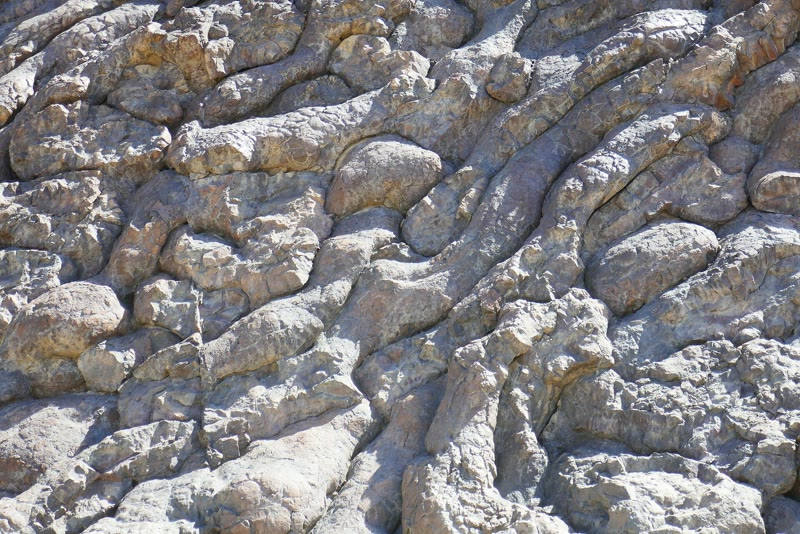
\includegraphics[width=0.6\linewidth]{images/book2/g12-duchoiselle-oman-pillows.jpg}

{\small Laves en coussins de l'\omterm{def:g12:mountain-building:ophiolite}{ophiolite} de Semail à Wadi Jizzi, en
Oman~: une lave refroidie sous l'eau en coussins arrondis, aujourd'hui à
l'air libre. Photographie Lionel Duchoiselle (CC~BY-SA~3.0).}
\end{omfigure}
% ledger: photo:g12-oman-pillows

\section{Raccourcir la croûte}

Comprimé latéralement, un corps de roche se casse s'il est froid et
cassant~; s'il est assez chaud pour se comporter de façon plastique, il se
plisse. Une chaîne de montagnes est pleine de \omterm{def:g12:mountain-building:fold}{plis} comme de failles.
% ledger: earle:folds

\subsection{Les plis}

\begin{definition}[Pli~; anticlinal~; synclinal~; axe du pli]\label{def:g12:mountain-building:fold}
Un \emph{pli}\index{pli} est une courbure de couches de roches. Ses côtés
inclinés sont les \emph{flancs}~; ils se rejoignent à la
\emph{charnière}, là où les couches sont le plus courbées, et la ligne qui
suit la charnière est l'\emph{axe du pli}\index{axe du pli}. Un
\emph{anticlinal}\index{anticlinal} est un pli dont les couches se
courbent vers le haut, ses flancs plongeant en s'écartant de l'axe~; un
\emph{synclinal}\index{synclinal} est un pli dont les couches se courbent
vers le bas, ses flancs plongeant vers l'axe.
\end{definition}
% ledger: earle:folds, tulane:fold-geometry

Le plan qui passe par les charnières des couches successives est le plan
axial. Anticlinaux et synclinaux vont en général par paires, le flanc de
l'un étant le flanc du suivant. Les \omterm{def:g12:mountain-building:fold}{plis} ont toutes les tailles, du
microscopique à plusieurs dizaines de kilomètres. Une fois érodé, un
\omterm{def:g12:mountain-building:fold}{anticlinal} montre ses couches les plus anciennes en son cœur, et un
\omterm{def:g12:mountain-building:fold}{synclinal} ses couches les plus jeunes~; un \omterm{def:g12:mountain-building:fold}{anticlinal} n'est pas forcément
une crête, ni un \omterm{def:g12:mountain-building:fold}{synclinal} une vallée, car l'érosion suit les couches dures
et tendres plutôt que la forme du \omterm{def:g12:mountain-building:fold}{pli}.
% ledger: earle:folds, tulane:fold-geometry

\begin{omfigure}
\begin{tikzpicture}[x=1.2cm, y=1.2cm, font=\scriptsize]
  \def\W{6}\def\H{2.0}\def\dx{1.35}\def\dy{0.78}
  \tikzset{declare function={zb(\x,\c)=\c+0.8*cos(60*(\x-1.5));}}
  \colorlet{bandA}{omLithSchist!70}\colorlet{bandB}{omLithSand}\colorlet{bandC}{omLithShale}
  \colorlet{bandD}{icsJurassic!35}\colorlet{bandE}{icsTriassic!35}\colorlet{bandF}{icsCretaceous!45}
  % front face
  \begin{scope}
    \clip (0,0) rectangle (\W,\H);
    \fill[bandA] (0,0) rectangle (\W,\H);
    \foreach \c/\col in {0.0/bandB, 0.6/bandC, 1.2/bandD, 1.8/bandE, 2.4/bandF}
      \fill[\col] plot[domain=0:\W, samples=80, smooth] (\x,{zb(\x,\c)}) -- (\W,4) -- (0,4) -- cycle;
    \foreach \c in {0.0,0.6,1.2,1.8,2.4}
      \draw[black!55, line width=0.35pt] plot[domain=0:\W, samples=80, smooth] (\x,{zb(\x,\c)});
  \end{scope}
  % top face: outcrop bands (crossings of the top surface computed for these curves)
  \fill[bandE] (0,\H) -- (0.242,\H) -- ++(\dx,\dy) -- (\dx,\H+\dy) -- cycle;
  \fill[bandD] (0.242,\H) -- (2.758,\H) -- ++(\dx,\dy) -- (0.242+\dx,\H+\dy) -- cycle;
  \fill[bandE] (2.758,\H) -- (3.5,\H) -- ++(\dx,\dy) -- (2.758+\dx,\H+\dy) -- cycle;
  \fill[bandF] (3.5,\H) -- (5.5,\H) -- ++(\dx,\dy) -- (3.5+\dx,\H+\dy) -- cycle;
  \fill[bandE] (5.5,\H) -- (\W,\H) -- ++(\dx,\dy) -- (5.5+\dx,\H+\dy) -- cycle;
  \foreach \x in {0.242,2.758,3.5,5.5} \draw[black!55, line width=0.35pt] (\x,\H) -- ++(\dx,\dy);
  % right face: the layers meet it at constant heights (cylindrical folds)
  \foreach \lo/\hi/\col in {0.0/0.6/bandB, 0.6/1.2/bandC, 1.2/1.8/bandD, 1.8/2.0/bandE}
    \fill[\col] (\W,\lo) -- (\W+\dx,\lo+\dy) -- (\W+\dx,\hi+\dy) -- (\W,\hi) -- cycle;
  \foreach \y in {0.6,1.2,1.8} \draw[black!55, line width=0.35pt] (\W,\y) -- ++(\dx,\dy);
  % outline
  \draw[black, line width=0.5pt] (0,0) rectangle (\W,\H) (0,\H) -- (\dx,\H+\dy) -- (\W+\dx,\H+\dy) -- (\W,\H)
    (\W+\dx,\H+\dy) -- (\W+\dx,\dy) -- (\W,0);
  % fold axes on the top face, axial planes on the front face
  \draw[omThm, line width=1pt] (1.5,\H) -- ++(\dx,\dy);
  \draw[omDef, line width=1pt] (4.5,\H) -- ++(\dx,\dy);
  \draw[omThm, dashed, line width=0.6pt] (1.5,0) -- (1.5,\H);
  \draw[omDef, dashed, line width=0.6pt] (4.5,0) -- (4.5,\H);
  \node[anchor=south, omThm] at (1.5+\dx,\H+\dy) {anticlinal~: axe du pli};
  \node[anchor=south, omDef] at (4.5+\dx,\H+\dy) {synclinal~: axe du pli};
  \draw[black!70] (3.2,0.95) -- (3.9,-0.35) node[anchor=north] {flanc};
  \draw[black!70] (1.5,1.4) circle (0.07) -- (0.4,-0.35) node[anchor=north] {charnière};
  \draw[black!70] (1.5,0.25) -- (2.0,-0.35) node[anchor=north] {plan axial};
\end{tikzpicture}

{\small Un \omterm{def:g12:mountain-building:fold}{anticlinal} et un \omterm{def:g12:mountain-building:fold}{synclinal} recoupés par une surface d'érosion
plane (bloc-diagramme sans échelle). Les axes des \omterm{def:g12:mountain-building:fold}{plis} suivent les
charnières~; les tirets sont les traces des plans axiaux. Sur la surface
du haut, l'\omterm{def:g12:mountain-building:fold}{anticlinal} érodé montre des couches plus anciennes en son cœur,
le \omterm{def:g12:mountain-building:fold}{synclinal} des couches plus jeunes.}
\end{omfigure}
% ledger: earle:folds, tulane:fold-geometry

\begin{omfigure}
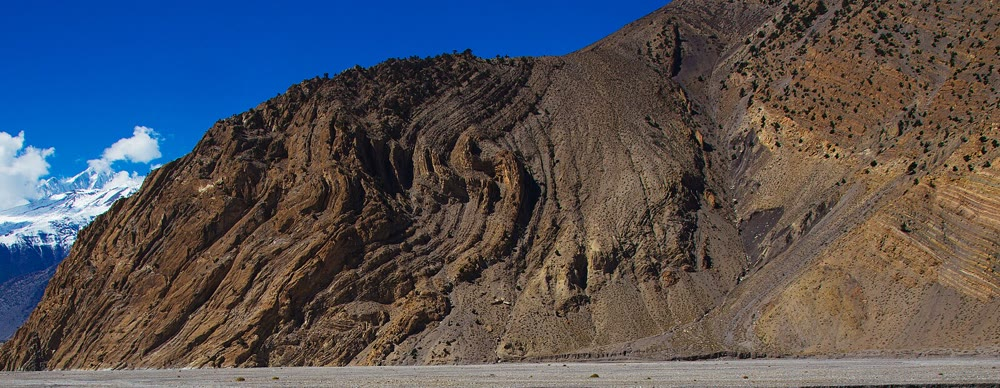
\includegraphics[width=0.95\linewidth]{images/book2/g12-hullot-kali-gandaki-folds.jpg}

{\small Des couches de roches plissées dans une falaise de l'Himalaya, à
environ \qty{3}{km} au nord-est de Jomsom, dans les gorges de la Kali
Gandaki, au Népal. Photographie Jean-Marie Hullot (CC~BY~2.0).}
\end{omfigure}
% ledger: photo:g12-kali-gandaki

La couverture des collines de Varden est plissée de la même façon, bien
plus doucement. Son grès, son calcaire, son argilite et sa craie se sont
déposés à plat, puis ont été courbés en un \omterm{def:g12:mountain-building:fold}{anticlinal} et un \omterm{def:g12:mountain-building:fold}{synclinal} dont
les flancs plongent de \ang{12}~; une \omterm{def:g11:ocean-ridges:normal-fault}{faille normale} plus récente les
recoupe.
% ledger: region:name; model in figdata/shared/region.py (LIMB_DIP 12, AXIS_ANTI 3.5 km, AXIS_SYN 7.5 km)

\begin{omfigure}
\begin{tikzpicture}
\begin{axis}[omsection, x=1.25cm, y=0.003125cm, xmin=0, xmax=9.49, ymin=-700, ymax=650,
  xlabel={distance à A (\unit{km})}, ylabel={altitude (\unit{m})},
  ytick={-600,-300,0,300,600}, tick label style={font=\scriptsize}]
\addplot[fill=black!8, draw=black!50, line width=0.3pt, even odd rule] table {figdata/out/shared-region-section-unit-schist.dat};
\addplot[fill=icsTriassic!20, draw=black!50, line width=0.3pt, even odd rule] table {figdata/out/shared-region-section-unit-sandstone.dat};
\addplot[fill=icsJurassic!25, draw=black!50, line width=0.3pt, even odd rule] table {figdata/out/shared-region-section-unit-limestone.dat};
\addplot[fill=icsJurassic!8, draw=black!50, line width=0.3pt, even odd rule] table {figdata/out/shared-region-section-unit-shale.dat};
\addplot[fill=icsCretaceous!20, draw=black!50, line width=0.3pt, even odd rule] table {figdata/out/shared-region-section-unit-chalk.dat};
\addplot[fill=omLithAlluv, draw=black!50, line width=0.3pt, even odd rule] table {figdata/out/shared-region-section-unit-alluvium.dat};
\addplot[black, line width=0.7pt] table {figdata/out/shared-region-section-ground.dat};
\addplot[fault] table {figdata/out/shared-region-section-fault.dat};
% axis positions from figdata/grade-12/fold_shortening.py (section_anticline_km, section_syncline_km; the syncline lies on the hanging wall, shifted by the fault heave)
\draw[omThm, dashed, line width=0.7pt] (axis cs:3.162,-700) -- (axis cs:3.162,660);
\draw[omDef, dashed, line width=0.7pt] (axis cs:7.484,-700) -- (axis cs:7.484,660);
\node[anchor=south, omThm, font=\scriptsize] at (axis cs:3.162,660) {axe de l'anticlinal};
\node[anchor=south, omDef, font=\scriptsize] at (axis cs:7.484,660) {axe du synclinal};
\node[anchor=south east, font=\small\bfseries] at (axis cs:0,650) {A};
\node[anchor=south west, font=\small\bfseries] at (axis cs:9.49,650) {B};
\node[font=\scriptsize, fill=white, inner sep=1pt] at (axis cs:1.2,-520) {schiste};
\node[font=\scriptsize, fill=white, inner sep=1pt, anchor=east] at (axis cs:6.55,-450) {faille normale};
\end{axis}
\end{tikzpicture}

\smallskip
{\small\tikz\fill[black!8, draw=black!50] (0,0) rectangle (0.35,0.22);~schiste \quad
\tikz\fill[icsTriassic!20, draw=black!50] (0,0) rectangle (0.35,0.22);~grès \quad
\tikz\fill[icsJurassic!25, draw=black!50] (0,0) rectangle (0.35,0.22);~calcaire \quad
\tikz\fill[icsJurassic!8, draw=black!50] (0,0) rectangle (0.35,0.22);~argilite \quad
\tikz\fill[icsCretaceous!20, draw=black!50] (0,0) rectangle (0.35,0.22);~craie \quad
\omve{2.5}}

{\small Coupe A--B à travers les collines de Varden, du sud-ouest au
nord-est. La couverture repose sur le socle de schiste et elle est
plissée en un \omterm{def:g12:mountain-building:fold}{anticlinal} et un \omterm{def:g12:mountain-building:fold}{synclinal}~; la \omterm{def:g11:ocean-ridges:normal-fault}{faille normale}, plus récente
que les \omterm{def:g12:mountain-building:fold}{plis}, abaisse le bloc nord-est. L'échelle verticale est étirée
2.5~fois, ce qui fait paraître les flancs plus raides qu'ils ne le sont.
Données~: le modèle de la région propre à la série.}
\end{omfigure}
% ledger: region:name; computed in figdata/shared/region.py (section A-B)

\subsection{Failles inverses, chevauchements et nappes}

Là où la croûte est comprimée alors qu'elle est froide et cassante, elle se
rompt le long de failles d'un autre type que les \omterm{def:g11:ocean-ridges:normal-fault}{failles normales} d'une
croûte étirée.

\begin{definition}[Faille inverse~; chevauchement]\label{def:g12:mountain-building:thrust}
Une \emph{faille inverse}\index{faille inverse} est une faille inclinée le
long de laquelle le bloc situé au-dessus du plan de faille est monté par
rapport au bloc situé au-dessous. Les failles inverses se forment là où la
croûte est comprimée. Un \emph{chevauchement}\index{chevauchement} est une
faille inverse à faible pendage, inférieur à \ang{45}.
\end{definition}
% ledger: earle:reverse-thrust, tulane:fold-geometry

Un \omterm{def:g12:mountain-building:thrust}{chevauchement} peut transporter une lame de roches sur des dizaines de
kilomètres~: des roches plus anciennes viennent alors reposer sur des
roches plus jeunes, à l'inverse de l'ordre dans lequel elles se sont
déposées. Dans les montagnes Rocheuses, le chevauchement de McConnell a
poussé un empilement de roches sédimentaires épais d'environ \qty{800}{m}
sur quelque \qty{40}{km}, d'ouest en est~: un calcaire vieux d'environ 500
millions d'années repose aujourd'hui sur une pélite vieille d'environ 75
millions d'années.
% ledger: earle:reverse-thrust

\begin{definition}[Nappe de charriage]\label{def:g12:mountain-building:nappe}
Une \emph{nappe de charriage}\index{nappe de charriage} est une grande lame
de roches transportée sur une longue distance, souvent des dizaines de
kilomètres, par-dessus les roches sous-jacentes, le long d'un \omterm{def:g12:mountain-building:thrust}{chevauchement}
presque plat.
\end{definition}
% ledger: ngu:nappe, earle:reverse-thrust

Une \omterm{def:g12:mountain-building:nappe}{nappe de charriage} peut transporter des roches formées très loin,
voire des écailles de fond océanique~; elle peut elle-même être plissée, ses
couches renversées. Les chaînes de montagnes empilent les nappes les unes
sur les autres. L'érosion perce ensuite des trous dans une nappe, ouvrant
des fenêtres sur les roches du dessous, et en laisse des morceaux isolés
posés sur les roches plus jeunes.
% ledger: ngu:nappe

\begin{omfigure}
\begin{tikzpicture}[x=1.0cm, y=1.0cm, font=\scriptsize]
  % rocks in place (younger), flat-lying
  \fill[icsCretaceous!25] (0,-1.6) rectangle (12,-0.4);
  \fill[icsJurassic!25] (0,-1.6) rectangle (12,-1.1);
  \draw[black!50, line width=0.3pt] (0,-1.1) -- (12,-1.1);
  \fill[white] (5.6,-0.4) -- (6.2,-0.62) -- (6.8,-0.4) -- cycle;
  % the nappe (older rocks) above a nearly flat thrust, cut by erosion
  \fill[omLithSchist!80] (0.8,-0.4) .. controls (1.2,0.35) and (1.9,0.35) .. (2.3,-0.4) -- cycle;
  \fill[omLithSchist!80] (3.2,-0.4) .. controls (3.9,0.9) and (4.8,0.9) .. (5.6,-0.4) -- cycle;
  \fill[omLithSchist!80] (6.8,-0.4) .. controls (7.1,0.9) and (7.7,1.3) .. (8.4,1.25) -- (12,0.9) -- (12,-0.4) -- cycle;
  % ground surface
  \draw[black, line width=0.6pt] (0,-0.4) -- (0.8,-0.4) .. controls (1.2,0.35) and (1.9,0.35) .. (2.3,-0.4)
     -- (3.2,-0.4) .. controls (3.9,0.9) and (4.8,0.9) .. (5.6,-0.4) -- (6.2,-0.62) -- (6.8,-0.4)
     .. controls (7.1,0.9) and (7.7,1.3) .. (8.4,1.25) -- (12,0.9);
  % thrust traces (teeth on the block that moved over)
  \draw[thrust fault] (0.8,-0.4) -- (2.3,-0.4);
  \draw[thrust fault] (3.2,-0.4) -- (5.6,-0.4);
  \draw[thrust fault] (6.8,-0.4) -- (12,-0.4);
  \draw[-{Stealth[length=2mm]}, line width=0.9pt] (11.4,1.45) -- (9.6,1.6);
  \node[anchor=south] at (10.5,1.55) {mouvement de la nappe};
  \node at (9.9,0.3) {nappe~: roches plus anciennes};
  \node[fill=white, inner sep=1pt] at (2.0,-0.85) {roches en place~: plus jeunes};
  \draw[black!60] (1.55,0.0) -- (1.3,0.8) node[anchor=south] {lambeau isolé};
  \draw[black!60] (6.2,-0.58) -- (6.2,-0.68) node[anchor=north, fill=white, inner sep=1pt] {fenêtre};
  \draw[black!60] (9.0,-0.42) -- (9.3,-0.68) node[anchor=north, fill=white, inner sep=1pt] {chevauchement};
\end{tikzpicture}

{\small Une \omterm{def:g12:mountain-building:nappe}{nappe de charriage} (sans échelle)~: une lame de roches plus
anciennes transportée le long d'un \omterm{def:g12:mountain-building:thrust}{chevauchement} presque plat par-dessus
des roches plus jeunes restées en place. L'érosion y a percé une fenêtre et
en a laissé un morceau isolé à gauche. Les dents du
\omterm{def:g12:mountain-building:thrust}{chevauchement} pointent vers le bloc qui est passé par-dessus.}
\end{omfigure}
% ledger: ngu:nappe, earle:reverse-thrust

\begin{omfigure}
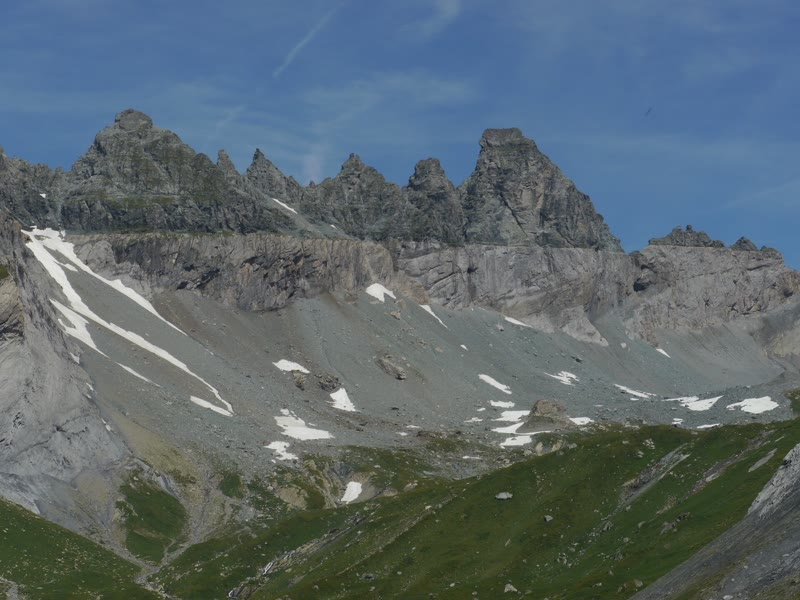
\includegraphics[width=0.5\linewidth]{images/book2/g12-heine-glarus-thrust.jpg}

{\small Le chevauchement de Glaris, dans les Alpes de l'est de la Suisse.
Les roches sombres des sommets, déposées au Permien, il y a environ 299 à
252 millions d'années, reposent sur des roches plus claires et bien plus
jeunes~; le \omterm{def:g12:mountain-building:thrust}{chevauchement} est la limite nette qui les sépare. Les roches du
dessus se sont déplacées de quelque 40 à \qty{50}{km}. Photographie
Christian Heine (CC~BY-SA~3.0).}
\end{omfigure}
% ledger: photo:g12-glarus (Verrucano, Permian; displacement 40-50 km, Pfiffner 1985), ics:base.Permian, ics:base.Triassic

\subsection{Mesurer le raccourcissement}

Les \omterm{def:g12:mountain-building:fold}{plis} comme les \omterm{def:g12:mountain-building:thrust}{chevauchements} raccourcissent la croûte dans la
direction où elle est comprimée.

\begin{definition}[Raccourcissement]\label{def:g12:mountain-building:shortening}
Le \emph{raccourcissement}\index{raccourcissement} d'une couche est la
fraction de sa longueur qu'elle a perdue~: si elle était longue de $L_0$
et s'étend aujourd'hui sur $L$,
\[
  e = \frac{L_0 - L}{L_0}.
\]
\end{definition}

Pour le mesurer, il faut connaître la longueur initiale $L_0$. Dans
beaucoup de \omterm{def:g12:mountain-building:fold}{plis}, les couches gardent leur épaisseur en se courbant, en
glissant les unes sur les autres comme les pages d'un livre que l'on
courbe~; une telle couche n'est pas étirée dans sa longueur. Cela donne la
longueur initiale.
% ledger: tulane:fold-geometry (flexural folds keep their thickness)

\begin{proposition}[Le raccourcissement d'une couche plissée]\label{prop:g12:mountain-building:shortening}
Si une couche s'est plissée sans être étirée ni comprimée dans sa
longueur, sa longueur initiale $L_0$ est sa longueur mesurée le long de la
couche plissée. Pour un \omterm{def:g12:mountain-building:fold}{pli} à flancs droits plongeant d'un angle $\theta$,
\[
  e = 1 - \cos\theta .
\]
\end{proposition}

\begin{proof}
Déplier la couche, sans l'étirer, l'étale à plat sans changer sa
longueur~; $L_0$ est donc la longueur mesurée le long de la couche. Sur un
flanc droit de longueur $\ell$ plongeant de $\theta$, la distance
horizontale parcourue est $\ell\cos\theta$ (triangle rectangle). En
ajoutant tous les flancs, la couche de longueur $L_0$ s'étend sur
$L = L_0\cos\theta$, et $e = (L_0 - L_0\cos\theta)/L_0 =
1 - \cos\theta$.
\end{proof}

\begin{omfigure}
\begin{tikzpicture}
\begin{axis}[name=sine, x=2.0cm, y=2.0cm, axis lines=none,
  xmin=-0.05, xmax=2.25, ymin=-0.4, ymax=0.8, clip=false]
% computed in figdata/grade-12/fold_shortening.py (part sine: A/lambda = 0.25, e = 31.7 %)
\addplot[omLithSand!80!black, line width=1.6pt] table[x=x, y=y] {figdata/out/grade-12-fold_shortening-sine.dat};
\draw[omThm, line width=1.6pt] (axis cs:0,0.62) -- (axis cs:2.196,0.62);
\draw[black!60, |-|] (axis cs:0,-0.32) -- node[below, font=\scriptsize] {$L$ (aujourd'hui)} (axis cs:1.5,-0.32);
\node[anchor=south west, font=\scriptsize, omThm] at (axis cs:0,0.64) {$L_0$~: la même couche dépliée};
\end{axis}
\begin{axis}[omrecord, at={(sine.east)}, anchor=west, xshift=1.4cm, width=0.46\linewidth, height=4.6cm,
  xmin=0, xmax=80, ymin=0, ymax=85, xlabel={pendage des flancs $\theta$ (\unit{\degree})},
  ylabel={raccourcissement $e$ (\unit{\percent})}, xtick={0,20,...,80}]
% computed in figdata/grade-12/fold_shortening.py (part dip: e = 1 - cos theta)
\addplot[omProp, line width=1pt] table[x=theta, y=e_pct] {figdata/out/grade-12-fold_shortening-dip.dat};
\addplot[only marks, mark=*, mark size=1.6pt, omThm] coordinates {(12,2.185) (30,13.397) (60,50)};
\node[anchor=south, font=\scriptsize, align=center] at (axis cs:12,6) {Varden~:\\\qty{2.2}{\percent}};
\node[anchor=west, font=\scriptsize] at (axis cs:32,10) {\qty{13}{\percent}};
\node[anchor=south east, font=\scriptsize] at (axis cs:60,51) {\qty{50}{\percent}};
\end{axis}
\end{tikzpicture}

{\small À gauche~: une couche plissée s'étend sur $L$~; étalée à plat, sans
être étirée, elle est longue de $L_0$ (ici, les \omterm{def:g12:mountain-building:fold}{plis} sont aussi hauts que
le quart de leur longueur d'onde, et $L$ vaut \qty{68}{\percent} de
$L_0$). À droite~: le \omterm{def:g12:mountain-building:shortening}{raccourcissement} d'un \omterm{def:g12:mountain-building:fold}{pli} à flancs droits,
$1 - \cos\theta$, en fonction du pendage de ses flancs. Des \omterm{def:g12:mountain-building:fold}{plis} doux
raccourcissent très peu une couche.}
\end{omfigure}
% values: sine_025_e_pct 31.68 (L/L0 = 0.683); varden_e_pct 2.1852; chevron_30 13.397; chevron_60 50 (fold_shortening.py)

\begin{method}[Mesurer le raccourcissement sur une coupe]\label{met:g12:mountain-building:shortening}
\begin{enumerate}
  \item Vérifier que la coupe est dessinée à l'échelle vraie. Si son
        échelle verticale est étirée, les pendages et les longueurs le long
        des couches sont trop grands~: la redessiner, ou corriger d'abord
        chaque pendage.
  \item Choisir une limite de couche que l'on peut suivre d'un bout à
        l'autre de la coupe~; là où une faille la coupe, raccorder les deux
        extrémités coupées comme elles l'étaient avant le jeu de la faille.
  \item Mesurer sa longueur le long de la couche, $L_0$~: la suivre avec un
        fil, ou additionner de courts segments droits.
  \item Mesurer la distance horizontale entre ses deux extrémités, $L$.
  \item Calculer $e = (L_0 - L)/L_0$~; pour des flancs droits de pendage
        connu, $e = 1 - \cos\theta$ le donne directement.
\end{enumerate}
\end{method}

\begin{example}[Les plis de Varden]\label{ex:g12:mountain-building:varden}
Les flancs des \omterm{def:g12:mountain-building:fold}{plis} de Varden plongent de \ang{12}~: la couverture a donc
été raccourcie de $e = 1 - \cos\ang{12} = 1 - 0.978 = 0.022$, environ
\qty{2.2}{\percent}~: une bande de la région large aujourd'hui de
\qty{10}{km} était large de $10/\cos\ang{12} \approx
\qty{10.22}{km}$ avant le plissement. Mesurés sur la coupe A--B telle
qu'elle est dessinée, les flancs paraîtraient plonger d'environ \ang{28},
car l'échelle verticale est étirée 2.5~fois~: $\tan\theta$ est multipliée
par 2.5, et $\arctan(2.5
\tan\ang{12}) \approx \ang{28}$. Pris pour argent comptant, cela donnerait
un \omterm{def:g12:mountain-building:shortening}{raccourcissement} de \qty{12}{\percent}, plus de cinq fois trop.
\end{example}
% values: varden_e_pct 2.1852, varden_L0_for_10km 10.223 (fold_shortening.py); arctan(2.5 x 0.2126) = 27.98 deg; 1 - cos 27.98 = 0.117

Les \omterm{def:g12:mountain-building:fold}{plis} doux absorbent peu. Une chaîne aux \omterm{def:g12:mountain-building:fold}{plis} serrés, dont les flancs
plongent de \ang{60}, a été raccourcie de moitié~; et un seul \omterm{def:g12:mountain-building:thrust}{chevauchement}
presque plat qui a transporté une nappe sur \qty{40}{km} absorbe
\qty{40}{km} de \omterm{def:g12:mountain-building:shortening}{raccourcissement}, autant qu'une très large bande de \omterm{def:g12:mountain-building:fold}{plis}
doux.

\section{Épaississement et soulèvement}

Le \omterm{def:g12:mountain-building:shortening}{raccourcissement} ne détruit pas la roche. Une bande de croûte comprimée
jusqu'à une fraction de sa largeur initiale garde son volume~: elle doit
donc s'épaissir. Si une croûte épaisse de $H_0$ est raccourcie d'une
largeur $L_0$ à une largeur $L$ sur toute la longueur de la chaîne, sa
section garde son aire, $H L = H_0 L_0$, et
\[
  H = H_0\,\frac{L_0}{L} = \frac{H_0}{1 - e}.
\]
Une croûte épaisse de \qty{35}{km} raccourcie de \qty{50}{\percent} devient
épaisse de \qty{70}{km}. L'\omterm{def:g11:lithosphere-asthenosphere:isostasy}{isostasie} fait alors le reste~: une croûte plus
épaisse flotte plus haut, au-dessus d'une \omterm{def:g12:continental-crust:root}{racine} plus profonde
(\cref{prop:g11:lithosphere-asthenosphere:airy}). Avec le modèle d'Airy et
les masses volumiques du rappel, une croûte plus épaisse de $\Delta H$ se
dresse plus haut de $\Delta H\,(\rho_m - \rho_c)/\rho_m = \Delta H
\times 550/3380$, environ un sixième du surcroît d'épaisseur~; les cinq
autres sixièmes forment la \omterm{def:g12:continental-crust:root}{racine}. La croûte est épaisse de 35 à
\qty{40}{km} loin des chaînes de montagnes, et de 50 à \qty{70}{km} sous
elles~: plus les montagnes sont hautes, plus la croûte est épaisse.
% ledger: tulane:roots, cm95:crust, data:prem

C'est ainsi que le calcaire d'un fond marin est arrivé au sommet de
l'Everest~: déposé au fond d'une mer, il a été emporté vers le nord avec
l'Inde, empilé dans les écailles chevauchantes de l'Himalaya, et soulevé à
mesure que la croûte située sous lui s'épaississait et montait. Un tel
mouvement vertical de la croûte s'appelle un soulèvement.
% ledger: sakai05:summit, sakai05:stacking, tulane:roots (uplift), usgs:himalaya-collision

\section{Deux chaînes}

\subsection{L'Himalaya}

L'Himalaya s'étend sur \qty{2900}{km} le long de la frontière entre l'Inde
et le Tibet. Il y a environ 80 millions d'années, l'Inde se trouvait à
quelque \qty{6400}{km} au sud de l'Asie, de l'autre côté d'un océan, et se
déplaçait vers le nord à environ \qty{9}{cm} par an~; elle a rencontré
l'Asie il y a 40 à 50 millions d'années, et sa progression vers le nord a
alors ralenti. Les reconstitutions des plaques retracent ce voyage en
détail~: construites à partir de nombreux types d'indices, parmi lesquels
les \omterm{def:g11:plate-motions:hotspot-track}{traces des points chauds} (\cref{ch:g11:plate-motions}), elles ramènent
les plaques en arrière dans le temps, étape par étape.
% ledger: usgs:himalaya-collision, muller19:frame, muller22:frame

\begin{omfigure}
\begin{tikzpicture}
\begin{axis}[omrecord, omage, name=lat, width=0.5\linewidth, height=5.2cm,
  xmin=0, xmax=100, ymin=-45, ymax=35, xlabel={âge (\unit{Ma})}, ylabel={latitude (\unit{\degree})},
  xtick={0,20,...,100}, ytick={-40,-20,...,40},
  legend style={font=\scriptsize, at={(0.98,0.03)}, anchor=south east, fill=white}]
% computed in figdata/grade-12/india_drift.py (part lat; GPlates Web Service, MULLER2022 and MULLER2019)
\fill[omThm!12] (axis cs:40,-45) rectangle (axis cs:50,35);
\addplot[omThm, line width=1.1pt] table[x=age, y=m22_india] {figdata/out/grade-12-india_drift-lat.dat};
\addplot[omThm, dashed, line width=0.8pt] table[x=age, y=m19_india] {figdata/out/grade-12-india_drift-lat.dat};
\addplot[omDef, line width=1.1pt] table[x=age, y=m22_lhasa] {figdata/out/grade-12-india_drift-lat.dat};
\addplot[black!50, line width=0.4pt, forget plot] coordinates {(0,0) (100,0)};
\legend{{Inde centrale (2022)}, {Inde centrale (2019)}, {Lhassa (2022)}}
\end{axis}
\begin{axis}[omrecord, omage, at={(lat.east)}, anchor=west, xshift=1.9cm, width=0.42\linewidth, height=5.2cm,
  xmin=0, xmax=100, ymin=0, ymax=160, xlabel={âge (\unit{Ma})},
  ylabel={vitesse vers le nord (\unit{mm/an})}, xtick={0,20,...,100}]
% computed in figdata/grade-12/india_drift.py (part steps: 5-Myr steps)
\fill[omThm!12] (axis cs:40,0) rectangle (axis cs:50,160);
\addplot[omThm, line width=1pt] table[x=age, y=m22] {figdata/out/grade-12-india_drift-steps.dat};
\addplot[omThm, dashed, line width=0.7pt] table[x=age, y=m19] {figdata/out/grade-12-india_drift-steps.dat};
\end{axis}
\end{tikzpicture}

{\small À gauche~: la latitude d'un point du centre de l'Inde (\ang{78}~E,
\ang{20}~N aujourd'hui) et de Lhassa, au nord de la \omterm{def:g12:mountain-building:suture}{suture}, au cours des
100 derniers millions d'années, dans deux reconstitutions des plaques
publiées (2022 et 2019). À droite~: la vitesse de l'Inde vers le nord dans
chaque étape de 5 millions d'années. La bande grisée marque l'intervalle
d'il y a 50 à 40 millions d'années. Données~: R.~D.~Müller et ses
collègues (2019, 2022), calcul avec le GPlates Web Service.}
\end{omfigure}
% ledger: data:b2-gws-india, muller22:frame, muller19:frame; values: speed_65_50 128.5, speed_40_0 40.06, fastest 145.8 (50-55 Ma) (india_drift.py)

Les deux reconstitutions concordent à quelques degrés près. Entre 65 et 50
millions d'années, l'Inde s'est déplacée vers le nord à environ
\qty{13}{cm} par an~; entre 50 et 40 millions d'années, sa vitesse a
chuté, et depuis 40 millions d'années elle se déplace à environ
\qty{4}{cm} par an, moins d'un tiers de sa vitesse passée. Lhassa, du côté
asiatique, s'est aussi déplacée vers le nord, mais bien plus lentement.
% values: speed_65_50 128.5 mm/yr, speed_40_0 40.06 mm/yr, slowdown_ratio 0.312 (india_drift.py)

\begin{example}[La vitesse de l'Inde]\label{ex:g12:mountain-building:india}
Dans la reconstitution de 2022, le centre de l'Inde se trouvait à
\ang{12.10}~S il y a 60 millions d'années et à \ang{0.68}~S il y a 50
millions d'années. Un degré de latitude vaut
$2\pi R/360 = 2\pi \times \qty{6371}{km}/360 \approx \qty{111.2}{km}$.
L'Inde s'est déplacée vers le nord de
$(12.10 - 0.68) \times 111.2 \approx \qty{1270}{km}$ en 10 millions
d'années~: \qty{127}{km} par million d'années, c'est-à-dire $\qty{127e6}{mm} /
\num{e6}\text{ ans} = \qty{127}{mm}$, environ \qty{13}{cm}, par an.
\end{example}
% ledger: data:b2-gws-india, earth:Rmean; values: lat 60 Ma -12.0964, 50 Ma -0.6801 (india_drift-lat)

Le ralentissement est interprété comme la marque de la collision~: la
\omterm{def:g12:continental-crust:continental-crust}{croûte continentale} qui arrivait à la fosse ne pouvait pas s'enfoncer, et
l'Inde a été freinée. La date exacte du premier contact est encore
débattue~: les estimations vont d'environ 60 à 54 millions d'années, et
certains géologues soutiennent que l'Inde a d'abord rencontré une chaîne
d'îles volcaniques et n'a atteint l'Asie elle-même qu'il y a environ 34
millions d'années. L'Inde ne s'est pas arrêtée~: les pôles de rotation des
plaques actuelles la déplacent vers l'Eurasie à environ \qty{4.5}{cm} par
an à travers l'Himalaya (\cref{ch:g11:plate-motions}), et la poussée chasse
des parties de l'Asie vers l'est.
% ledger: usgs:himalaya-collision, najman21:collision-age; values: today_in_eu_speed 44.99 mm/yr (india_drift.py, from nnr56:poles)

Au nord de l'Himalaya, le plateau du Tibet culmine en moyenne à environ
\qty{4600}{m}, au-dessus d'une croûte épaisse d'environ \qty{70}{km}
(\cref{ch:g11:lithosphere-asthenosphere}). Entre l'Inde et le Tibet
s'étend la \omterm{def:g12:mountain-building:suture}{suture} de l'Indus--Tsangpo et ses \omterm{def:g12:mountain-building:ophiolite}{ophiolites}~; au sud de
celle-ci, l'Himalaya est fait en grande partie de sédiments déposés sur la
bordure nord de l'Inde, puis empilés, plissés et faillés, le calcaire du
sommet de l'Everest parmi eux.
% ledger: karplus:tibet-moho, liu20:itsz, sakai05:stacking, sakai05:summit; Book 1: usgs:himalaya (Tibetan Plateau about 4600 m)

\subsection{Les Alpes, et toute une ceinture}

Les Alpes ont une histoire semblable, à une échelle plus petite~: elles se
sont élevées là où l'Afrique est entrée en collision avec l'Europe. Elles
aussi contiennent des \omterm{def:g12:mountain-building:ophiolite}{ophiolites}, et de grands \omterm{def:g12:mountain-building:thrust}{chevauchements}~: au
chevauchement de Glaris, des roches permiennes ont été transportées
par-dessus des roches bien plus jeunes. Les Alpes et l'Himalaya
appartiennent à une même longue ceinture de montagnes, qui passe par le
Zagros, en Iran, là où l'Afrique et l'Inde sont entrées en collision avec
l'Eurasie.
% ledger: earle:collision, photo:g12-glarus

\begin{omfigure}
\begin{tikzpicture}
\begin{axis}[axis equal image, xmin=-12, xmax=105, ymin=18, ymax=52, width=\linewidth,
  tick label style={font=\scriptsize}, xtick={0,30,60,90}, ytick={20,30,40,50},
  xticklabel={$\pgfmathprintnumber{\tick}^\circ$}, yticklabel={$\pgfmathprintnumber{\tick}^\circ$},
  axis background/.style={fill=omSea}, legend columns=3,
  legend style={font=\scriptsize, at={(0.5,-0.12)}, anchor=north, /tikz/every even column/.append style={column sep=5pt}}]
\addplot[fill=omLithAlluv, draw=black!45, line width=0.2pt, forget plot] table {figdata/out/shared-geo-land.dat};
% computed in figdata/grade-12/alpine_belt.py; ledger: data:etopo1, data:usgs-comcat
\addplot[only marks, mark=square*, mark size=1.15pt, omLithSand!85!black] table[x=lon, y=lat] {figdata/out/grade-12-alpine_belt-high.dat};
\addplot[only marks, mark=square*, mark size=1.15pt, omThm!75!black] table[x=lon, y=lat] {figdata/out/grade-12-alpine_belt-higher.dat};
\addplot[only marks, mark=*, mark size=0.7pt, black] table[x=lon, y=lat] {figdata/out/grade-12-alpine_belt-quakes.dat};
\addplot[omDef, line width=0.9pt, forget plot] table {figdata/out/shared-geo-school-collision.dat};
\addplot[black!70, line width=0.5pt, forget plot] table {figdata/out/shared-geo-school-subduction.dat};
\legend{{plus de \qty{1500}{m}}, {plus de \qty{3500}{m}}, {séisme de magnitude 6 ou plus}}
\coordinate (alps) at (axis cs:9,48);
\coordinate (zagros) at (axis cs:46,23.5);
\coordinate (zagrosbelt) at (axis cs:50.5,31.5);
\coordinate (himal) at (axis cs:84,24);
\coordinate (tibet) at (axis cs:88,33);
\coordinate (arrA) at (axis cs:77,19.5);
\coordinate (arrB) at (axis cs:79.2,25);
\end{axis}
% labels drawn after the axis, so that no earthquake dot covers them
\node[font=\scriptsize, fill=white, inner sep=1pt, anchor=south] at (alps) {Alpes};
\draw[black!60, line width=0.4pt] (zagros) -- (zagrosbelt);
\node[font=\scriptsize, fill=white, inner sep=1pt] at (zagros) {Zagros};
\node[font=\scriptsize, fill=white, inner sep=1pt, anchor=west] at (himal) {Himalaya};
\node[font=\scriptsize, fill=white, inner sep=1pt] at (tibet) {plateau du Tibet};
\draw[-{Stealth[length=2mm]}, line width=1pt, omProp] (arrA) -- (arrB);
\end{tikzpicture}

{\small La ceinture de montagnes jeunes de l'Atlantique au Tibet~: les
reliefs élevés (chaque carré est une maille de 1~degré), les séismes
superficiels de magnitude 6 ou plus de 1976 à 2025 (à moins de
\qty{70}{km} de profondeur), et les limites de collision entre plaques
(trait bleu). La flèche montre le mouvement de l'Inde vers l'Eurasie.
Données~: ETOPO1, catalogue des séismes de l'USGS, limites de plaques de
Bird (2003), terres émergées d'après Natural Earth.}
\end{omfigure}
% ledger: data:etopo1, data:usgs-comcat, data:pb2002, data:ne-land; values: n_quakes 398 (alpine_belt.py)

Les reliefs élevés et les séismes suivent la même bande étroite. La
collision n'est pas terminée~: les séismes montrent que la croûte continue
de se rompre le long de toute la ceinture, et que les montagnes sont encore
en train de se former.

\section{Exercices}

\begin{exercise}[$\star$]\label{exo:g12:mountain-building:1}
Associer chaque terme à sa description~: \omterm{def:g12:mountain-building:fold}{anticlinal}, \omterm{def:g12:mountain-building:fold}{synclinal},
\omterm{def:g12:mountain-building:thrust}{chevauchement}, \omterm{def:g12:mountain-building:nappe}{nappe de charriage}, \omterm{def:g12:mountain-building:suture}{suture}, \omterm{def:g12:mountain-building:ophiolite}{ophiolite}. (a) une \omterm{def:g12:mountain-building:thrust}{faille
inverse} à faible pendage~; (b) un morceau de fond océanique trouvé sur la
terre ferme~; (c) un \omterm{def:g12:mountain-building:fold}{pli} dont les flancs plongent vers son axe~; (d) la
ligne où deux continents ont été réunis~; (e) un \omterm{def:g12:mountain-building:fold}{pli} dont les flancs
plongent en s'écartant de son axe~; (f) une grande lame de roches
transportée loin le long d'un \omterm{def:g12:mountain-building:thrust}{chevauchement}.
\end{exercise}

\begin{exercise}[$\star$]\label{exo:g12:mountain-building:2}
De part et d'autre d'une vallée, les couches du côté ouest plongent de
\ang{20} vers l'ouest et celles du côté est de \ang{20} vers l'est. (1) Le
\omterm{def:g12:mountain-building:fold}{pli} qui les sépare est-il un \omterm{def:g12:mountain-building:fold}{anticlinal} ou un \omterm{def:g12:mountain-building:fold}{synclinal}~? (2) Après
l'érosion, trouve-t-on le long de son axe les couches les plus anciennes ou
les plus jeunes~? (3) La vallée doit-elle se trouver au-dessus d'un
\omterm{def:g12:mountain-building:fold}{synclinal}~?
\end{exercise}

\begin{exercise}[$\star$]\label{exo:g12:mountain-building:3}
Une couche est plissée en flancs droits qui plongent de \ang{30}.
(1) Calculer son \omterm{def:g12:mountain-building:shortening}{raccourcissement}. (2) Elle s'étend aujourd'hui sur
\qty{6.0}{km}. Quelle était sa longueur~?
\end{exercise}

\begin{exercise}[$\star$]\label{exo:g12:mountain-building:4}
(1) Le long d'une faille, le bloc situé au-dessus du plan de faille est
descendu. S'agit-il d'une \omterm{def:g11:ocean-ridges:normal-fault}{faille normale} ou inverse, et la croûte a-t-elle
été étirée ou comprimée~? (2) Une \omterm{def:g12:mountain-building:thrust}{faille inverse} a un pendage de \ang{25}~:
est-ce un \omterm{def:g12:mountain-building:thrust}{chevauchement}~?
\end{exercise}

\begin{exercise}[$\star$]\label{exo:g12:mountain-building:5}
(1) Ranger de haut en bas ces roches d'une \omterm{def:g12:mountain-building:ophiolite}{ophiolite}~: \omterm{def:g11:ocean-ridges:gabbro}{gabbro}, sédiments
marins, \omterm{def:g11:ocean-ridges:peridotite}{péridotite}, basaltes en coussins, complexe filonien. (2) Pourquoi
les basaltes en coussins montrent-ils que la roche s'est formée sous
l'eau~? (3) Pourquoi trouve-t-on des \omterm{def:g12:mountain-building:ophiolite}{ophiolites} le long des \omterm{def:g12:mountain-building:suture}{sutures}~?
\end{exercise}

\begin{exercise}[$\star\star$]\label{exo:g12:mountain-building:6}
Sur une coupe à l'échelle vraie, on suit une limite de grès le long de
quatre segments droits longs de \qty{2.1}{km}, \qty{1.8}{km}, \qty{2.4}{km}
et \qty{1.6}{km}~; ses extrémités sont distantes de \qty{6.0}{km}.
(1) Calculer le \omterm{def:g12:mountain-building:shortening}{raccourcissement}. (2) Si les quatre flancs plongent tous du
même angle, quel est cet angle~?
\end{exercise}

\begin{exercise}[$\star\star$]\label{exo:g12:mountain-building:7}
Le bloc supérieur d'un \omterm{def:g12:mountain-building:thrust}{chevauchement} de pendage \ang{10} s'est déplacé de
\qty{45}{km} le long du plan de faille. (1) De combien s'est-il déplacé
horizontalement~? (2) De combien s'est-il élevé~? (3) Quelle largeur de
\omterm{def:g12:mountain-building:fold}{plis} aux flancs plongeant de \ang{12} absorberait le même \omterm{def:g12:mountain-building:shortening}{raccourcissement}
horizontal~?
\end{exercise}

\begin{exercise}[$\star\star$]\label{exo:g12:mountain-building:8}
Le long du chevauchement de McConnell, un calcaire vieux d'environ 500
millions d'années repose sur une pélite vieille d'environ 75 millions
d'années. (1) Quel principe de datation relative tromperait un géologue
qui ignorerait la faille~? (2) De combien la roche du dessus est-elle plus
ancienne~? (3) La lame chevauchante est épaisse d'environ \qty{800}{m} et
s'est déplacée de \qty{40}{km}~: combien de fois sa propre épaisseur cela
représente-t-il~?
\end{exercise}

\begin{exercise}[$\star\star$]\label{exo:g12:mountain-building:9}
Dans la reconstitution de 2022, le centre de l'Inde se trouvait à
\ang{30.23}~S il y a 80 millions d'années et à \ang{19.38}~S il y a 66
millions d'années. (1) De combien s'est-il déplacé vers le nord~? (2) À
quelle vitesse moyenne, en \unit{cm} par an~? (3) Comparer au résumé de
l'US Geological Survey, environ \qty{9}{m} par siècle.
\end{exercise}

\begin{exercise}[$\star\star$]\label{exo:g12:mountain-building:10}
Une croûte épaisse de \qty{35}{km} est raccourcie de \qty{40}{\percent} sur
toute une chaîne. (1) Quelle épaisseur atteint-elle~? (2) Avec $\rho_c =
\qty{2830}{kg/m^3}$ et $\rho_m = \qty{3380}{kg/m^3}$, de combien se
dresse-t-elle plus haut, et quelle est la profondeur de sa \omterm{def:g12:continental-crust:root}{racine}
supplémentaire~?
\end{exercise}

\begin{exercise}[$\star\star$]\label{exo:g12:mountain-building:11}
Sur une coupe dessinée avec une échelle verticale étirée 3~fois, un flanc
semble plonger de \ang{40}. (1) Quel est son pendage vrai~? (2) Calculer
le \omterm{def:g12:mountain-building:shortening}{raccourcissement} à partir du pendage vrai et à partir du pendage lu sur
le dessin. (3) Pourquoi les coupes servant à mesurer le \omterm{def:g12:mountain-building:shortening}{raccourcissement}
doivent-elles être dessinées à l'échelle vraie~?
\end{exercise}

\begin{exercise}[$\star\star\star$]\label{exo:g12:mountain-building:12}
Les \omterm{def:g12:mountain-building:fold}{plis} arrondis dessinés dans ce chapitre, aussi hauts que le quart de
leur longueur d'onde, ont un \omterm{def:g12:mountain-building:shortening}{raccourcissement} de \qty{31.7}{\percent}~; leur
pendage le plus fort est d'environ \ang{57.5}. (1) Une couche ainsi plissée
s'étend sur \qty{10}{km}~: quelle était sa longueur~? (2) Calculer le
\omterm{def:g12:mountain-building:shortening}{raccourcissement} d'un \omterm{def:g12:mountain-building:fold}{pli} à flancs droits de pendage \ang{57.5}.
(3) Expliquer pourquoi le \omterm{def:g12:mountain-building:fold}{pli} à flancs droits raccourcit davantage pour le
même pendage maximal.
\end{exercise}

\begin{exercise}[$\star\star\star$]\label{exo:g12:mountain-building:13}
Au nord de l'Himalaya, à \ang{85}~E \ang{28}~N, les pôles de rotation
donnent à l'Inde, par rapport à l'Eurasie, une vitesse de
\qty{16.6}{mm/an} vers l'est et de \qty{41.8}{mm/an} vers le nord. Sur les
5 derniers millions d'années, la reconstitution de 2022 donne au centre de
l'Inde une vitesse vers le nord supérieure de \qty{23.5}{mm/an} à celle de
Lhassa. (1) Trouver la vitesse de l'Inde par rapport à l'Eurasie.
(2) En admettant que les composantes nord puissent être comparées, quel
\omterm{def:g12:mountain-building:shortening}{raccourcissement} nord--sud par million d'années reste-t-il pour la région
située au nord de Lhassa~? (3) Où trouve-t-on dans le chapitre un signe que
cette région se déforme~?
\end{exercise}

\begin{exercise}[$\star\star\star$]\label{exo:g12:mountain-building:14}
Dans les Alpes, une \omterm{def:g12:mountain-building:nappe}{nappe de charriage} a été transportée sur \qty{45}{km}
le long d'un \omterm{def:g12:mountain-building:thrust}{chevauchement} de pendage presque nul. (1) Quel \omterm{def:g12:mountain-building:shortening}{raccourcissement}
ce \omterm{def:g12:mountain-building:thrust}{chevauchement} a-t-il absorbé~? (2) Quelle largeur, avant plissement,
d'une couverture plissée comme celle des collines de Varden (flancs à
\ang{12}) absorberait le même \omterm{def:g12:mountain-building:shortening}{raccourcissement}~? (3) Que montre ce calcul
sur la façon dont les chaînes de montagnes absorbent de grandes
convergences~?
\end{exercise}

\begin{exercise}[$\star\star\star$]\label{exo:g12:mountain-building:15}
Le calcaire du sommet de l'Everest s'est déposé sur un fond marin, au moins
un peu au-dessous du niveau de la mer, et se trouve aujourd'hui à
\qty{8848.86}{m}. (1) En admettant que la collision ait commencé il y a 50
millions d'années, quelle est la vitesse moyenne minimale du soulèvement, en
\unit{mm} par an~? (2) La comparer à la vitesse de l'Inde depuis 40 millions
d'années, environ \qty{40}{mm} par an. (3) Pourquoi le soulèvement de la
roche est-il probablement plus grand que son altitude actuelle~?
\end{exercise}

\begin{problem}[{Problème du week-end --- le voyage de l'Inde}]
\label{pb:g12:mountain-building:1}
% ledger: data:b2-gws-india, earth:Rmean, usgs:himalaya-collision, tulane:roots, cm95:crust, data:prem, karplus:tibet-moho; Book 1: usgs:himalaya (4600 m)
% values: india_drift-lat (MULLER2022, rounded to 0.01 deg); north_since_66_km 4378.7; converge_since_50 1354; gap_0 1073
Le tableau donne la latitude d'un point du centre de l'Inde et de Lhassa,
au nord de la \omterm{def:g12:mountain-building:suture}{suture}, dans la reconstitution des plaques de 2022 (valeur
négative = sud). Prendre un degré de latitude égal à \qty{111.2}{km}, et
\qty{1}{km} par million d'années égal à \qty{1}{mm} par an.

\begin{center}
\small
\begin{tabular}{|l|c|c|c|c|c|c|c|c|c|}
\hline
âge (\unit{Ma}) & 80 & 66 & 60 & 55 & 50 & 45 & 40 & 20 & 0 \\ \hline
Inde (\unit{\degree}) & $-30.23$ & $-19.38$ & $-12.10$ & $-7.24$ & $-0.68$ & 3.30 & 5.59 & 13.40 & 20.00 \\ \hline
Lhassa (\unit{\degree}) & & 19.48 & & & 21.15 & & & & 29.65 \\ \hline
\end{tabular}
\end{center}

\medskip
\noindent\textbf{Partie I --- Latitudes et vitesses.}
\begin{enumerate}
  \item Vérifier la valeur de \qty{111.2}{km} pour un degré, avec $R =
        \qty{6371}{km}$.
  \item Quand le centre de l'Inde a-t-il franchi l'équateur~?
  \item De combien l'Inde s'est-elle déplacée vers le nord entre 66 et 50
        millions d'années~?
  \item À quelle vitesse moyenne~?
  \item Calculer sa vitesse dans chaque étape entre 66 et 40 millions
        d'années (de 66 à 60, de 60 à 55, et ainsi de suite). Dans quelle
        étape était-elle la plus rapide~?
\end{enumerate}

\medskip
\noindent\textbf{Partie II --- Le ralentissement.}
\begin{enumerate}[resume]
  \item Calculer la vitesse moyenne de l'Inde entre il y a 40 millions
        d'années et aujourd'hui.
  \item Quelle fraction de sa vitesse entre 66 et 50 millions d'années
        cela représente-t-il~?
  \item Entre quelles dates du tableau la vitesse a-t-elle le plus chuté~?
  \item Pourquoi une collision ralentit-elle la plaque~?
  \item De combien l'Inde s'est-elle déplacée vers le nord entre il y a 50
        millions d'années et aujourd'hui~?
\end{enumerate}

\medskip
\noindent\textbf{Partie III --- La convergence absorbée.}
\begin{enumerate}[resume]
  \item De combien Lhassa s'est-elle déplacée vers le nord entre il y a 50
        millions d'années et aujourd'hui~?
  \item De combien la distance nord--sud entre le centre de l'Inde et
        Lhassa a-t-elle diminué depuis 50 millions d'années~?
  \item Quelle est cette distance aujourd'hui, et quelle était-elle il y a
        50 millions d'années~?
  \item Supposer que toute cette convergence a été absorbée par le
        \omterm{def:g12:mountain-building:shortening}{raccourcissement} de la croûte située entre les deux points. Quel
        est le \omterm{def:g12:mountain-building:shortening}{raccourcissement} $e$~?
  \item Nommer les deux types de structures qui absorbent un tel
        \omterm{def:g12:mountain-building:shortening}{raccourcissement}.
\end{enumerate}

\medskip
\noindent\textbf{Partie IV --- La croûte épaissie.}
\begin{enumerate}[resume]
  \item Si cette croûte était épaisse de \qty{35}{km} il y a 50 millions
        d'années, quelle serait son épaisseur aujourd'hui, en gardant sa
        section~?
  \item Avec $\rho_c = \qty{2830}{kg/m^3}$ et $\rho_m = \qty{3380}{kg/m^3}$,
        de combien se dresserait-elle au-dessus de son ancien niveau~?
  \item Le plateau du Tibet culmine à environ \qty{4600}{m}, au-dessus d'une
        croûte épaisse d'environ \qty{70}{km}. Quelle épaisseur de croûte le
        modèle d'Airy donne-t-il pour \qty{4600}{m}~?
  \item Donner une raison pour laquelle le modèle simple de la question~16
        surestime l'épaississement.
  \item En ajoutant les distances des questions~3 et~10, quelle distance
        l'Inde a-t-elle parcourue vers le nord depuis la fin du Crétacé, il
        y a 66 millions d'années~?
\end{enumerate}
\end{problem}
